
\chapter{Sinn und Zweck paralleler Programmierung}
\label{intro}
Seit Beginn der Rechentechnik Anfang der 40er Jahre verfolgen Informatiker das Ziel die zur Verfügung stehende Rechenleistung effizient zu nutzen.

Die parallele Programmierung stellt eine wesentliche Maßnahme dar, um dieses Ziel zu erreichen. Mit dieser Arbeit  soll die Umsetzung eines gegebenen Problems auf einer Grafikkarte mittels nVidia CUDA vorgestellt werden.

Parallele Programme beschreiben potentiell gleichzeitig ablaufende Aktivitäten, die miteinander kooperieren, um eine gemeinsame Aufgabe zu lösen. Dies setzt Programme voraus, die unabhängig von der Anzahl und der Geschwindigkeit der Prozessoren die gewünschten Ergebnisse liefern. Die Softwareentwicklung für parallele Algorithmen ist deshalb im Vergleich zur sequentiellen Programmierung wesentlich komplexer.

Durch die Aufteilung eines Programms in sogenannte \textbf{Threads} (\glqq leichtgewichtige Prozesse\grqq) lassen sich die Ressourcen heutiger Mirkoprozessoren effizient nutzen.
Threads besitzen dabei folgende Eigenschaften:
\begin{itemize}
\item sind sequentielle Befehlsausführungen
\item stellen Einheit für die Prozessorzuteilung dar
\item laufen in einem Prozessadressraum ab
\end{itemize}
Mit der Einführung von Threads werden im wesentlichen zwei Ziele verfolgt:
\begin{enumerate}
\item Strukturierung unabhängiger Programme und Programmkomponenten
\item Leistungssteigerung durch effiziente Parallelarbeit
\end{enumerate}

%Besonders aus der Möglichkeit der effizienten Parallelarbeit geht ein weiterer wesentlicher Vorteil hervor:
Die Leistungsfähigkeit von Programmen ist hauptsächlich abhängig von der Taktrate der CPU. Erhöht sich die Taktrate, wird ebenso das Programm schneller.
Allerdings haben die Taktraten heutiger CPUs einen Grenzwert erreicht.
Größere Taktraten würden diverse technische Probleme mit sich bringen, wie beispielsweise erhöhte Wärmeentwicklung auf dem Prozessor und damit verbundene, eine geeignete Wärmeabfuhr zu finden.
Daher gehen Chiphersteller schon seit einigen Jahren den Weg, möglichst viele Recheneinheiten (Kerne) auf einer CPU unterzubringen. Grafikprozessoren sind von Haus aus mit einer deutlich größeren Anzahl an Kernen ausgestattet.
Programme die entsprechend implementiert wurde diese Technologien effizient zu nutzen, können einen deutlichen Geschwindigkeitsvorteil gegenüber einer parallelen Ausführung auf einer CPU aufweisen.


\chapter{Aufgabenstellung}
Gegeben Kraft-Abstandskurven eines Rasterkraftmikroskops. Rasterkraftmikroskope werden zur Untersuchung von Oberflächen genutzt, um bspw. ein Höhenprofil erstellen zu können. Hierzu wird die vorliegende Oberfläche an möglichst vielen Stellen mit einer ca. 40 nm großen Spitze abgetastet, d.h. es wird zu jeder Messhöhe die der Abtastspitze entgegengebrachte Kraft gemessen.
Der Verlauf einer solchen Kraft-Abstandskurve lässt sich in drei lineare Funktionen unterteilen und ist qualitativ in Abbildung \ref{fig:kraftqual} dargestellt.

\begin{figure}[h!]
\centering
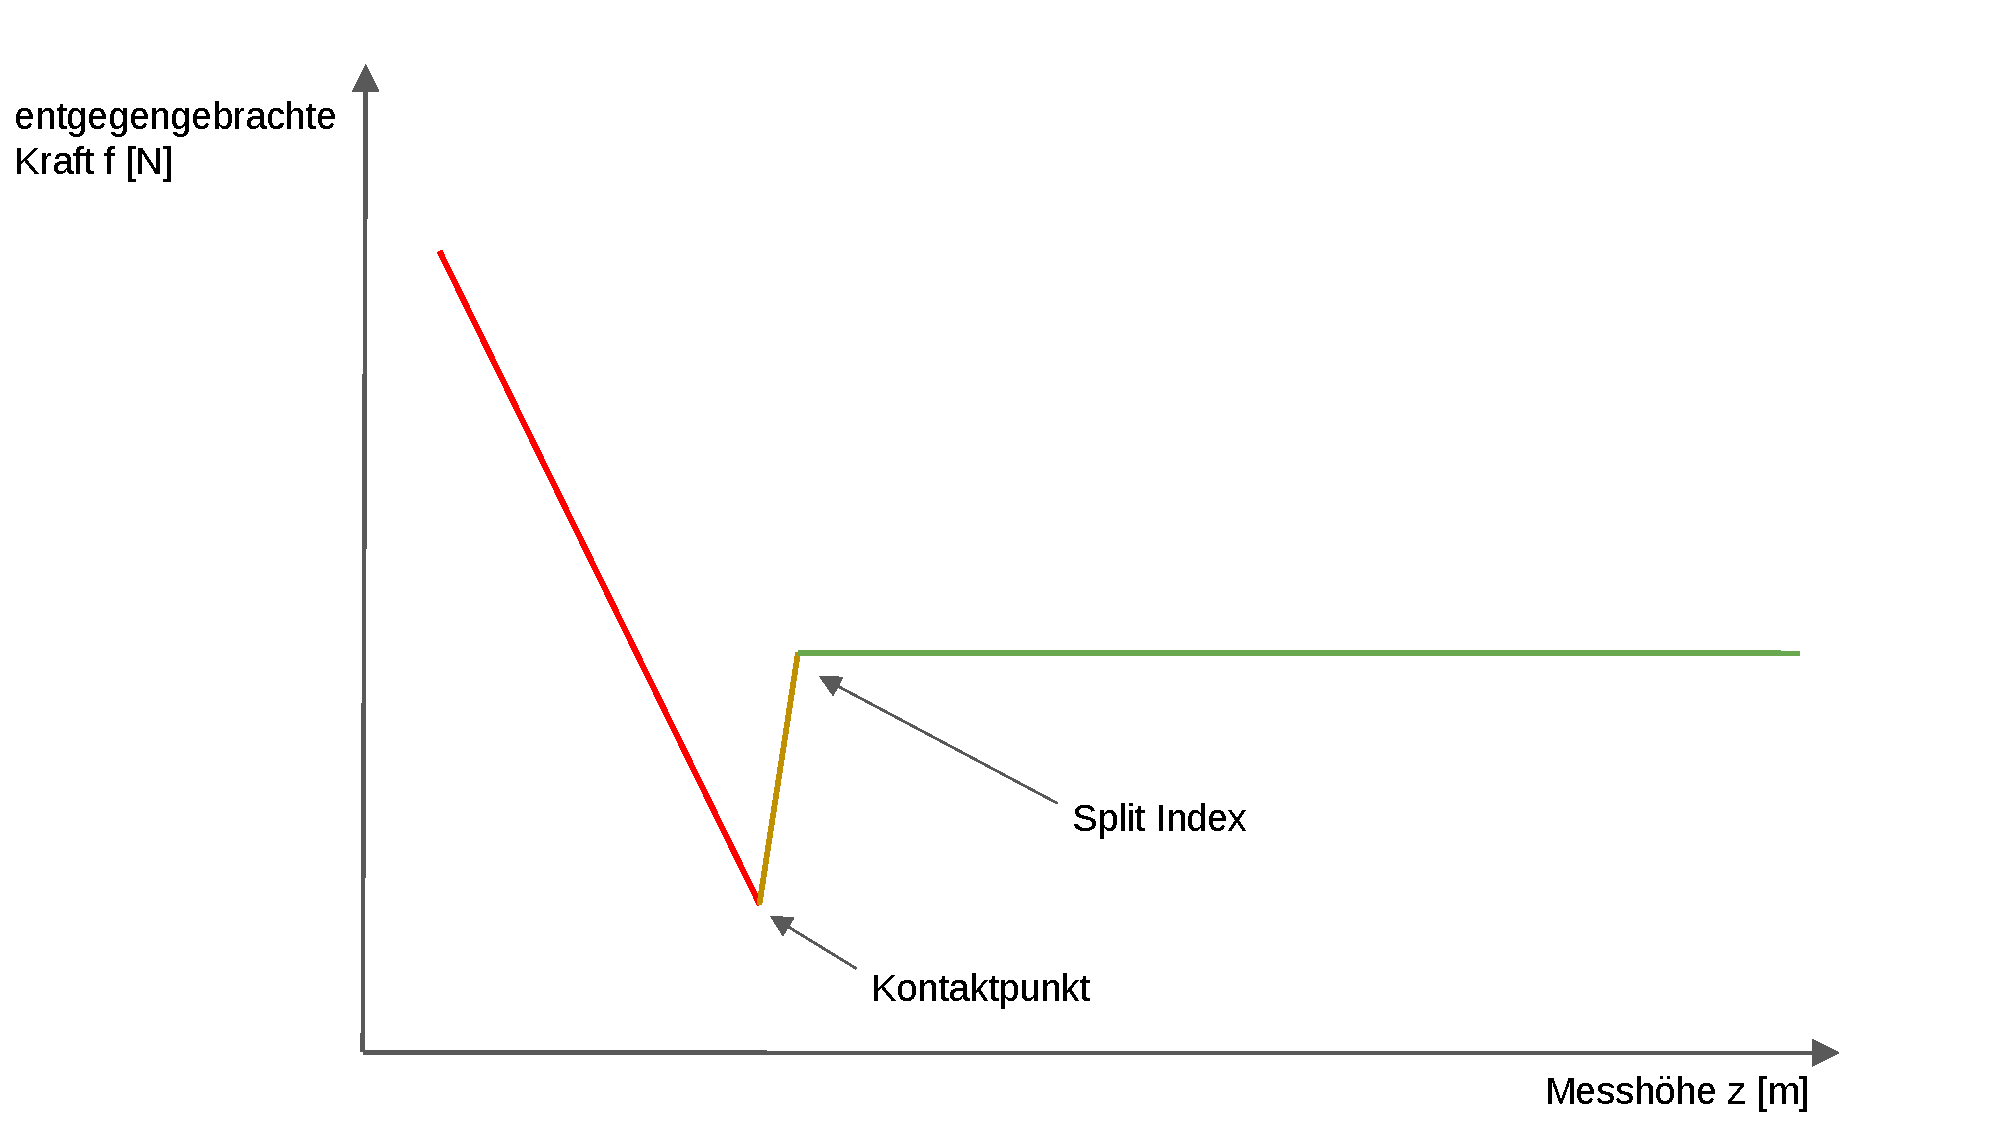
\includegraphics[scale=0.5]{qual.pdf}
\caption{Qualitativer Verlauf einer Kraft-Abstandskurve}
\label{fig:kraftqual}
\end{figure}

Der grüne Kurvenverlauf stellt die Annäherung der Abtastspitze zur Probe dar. Auffällig ist, dass die entgegengebrachte Kraft bei diesem Vorgang konstant bleibt.
Die gelbe Kurve zeigt, wie die Spitze von den Adhäsionskraften zwischen ihr und der Probe erfasst wird. Die entgegengebrachte Kraft fällt daher rapide ab, bis die Spitze Kontakt mit der Probe an der Stelle $c$ hergestellt hat.
Der rote Kurvenabschnitt zeigt, wie die auf die Spitze einwirkende Kraft nach Kontaktherstellung stark zunimmt, während weiterhin versucht wird, sich der Probe anzunähern.

Ziel ist es nun, die gegebene Punktewolke eines realen Rasterkraftmikroskops in diese drei linearen Funktionen zu zerlegen.
Ein Ausschnitt einer solchen realen Kraft-Abstandskurve ist in Abbildung \ref{fig:kraftbsp} dargestellt.


\begin{figure}[h!]
\centering
 \begin{tikzpicture}[scale=1]
 \begin{axis}[
   width=15cm,
   xlabel=Messhöhe in m,
   ylabel=Kraft in N]
 \addplot table [y=$Q_A$, x=P]{ex.txt};
 %\addlegendentry{$Q_A$ series}
 \end{axis}
 \end{tikzpicture}
\caption{Ausschnitt einer Kraft-Abstandskurve}
\label{fig:kraftbsp}
\end{figure}

Aufgenommen wurden solche Abtastungen an 256x*256y Positionen, wobei sowohl eine Messung für das Anfahren auf die Probe als auch das Ablassen von ihr aufgezeichnet wurde. Es liegen also insgesamt 131072 Datensätze vor, deren je 300 Abtastwerte mittels dreifach linearer Regression auf einer GPU in die oben beschriebene Form gebracht werden sollen, indem der Kontaktpunkt mit der Probe und der Splitindex gefunden werden.


\section{Einlesen der Datensätze}
Die Datensätze liegen als Textdeateien vor, wobei an jede Messposition in einer eigenen Datei gepsiechert ist. Es liegen somit 65536 Textdateien vor, in denen die Messwerte für das An-/ und Abfahren von der Probe zeilenweise ähnlich wie in einer CSV Datei gepseichert sind.
Das Einlesen dieser vielen 100KiB kleinen Dateien wird durch das häufige öffnen und schließen der Dateien und dem damit verbundenen Overhead seitens des Betreibssystems verlangsamt. Zudem werden für die nötigen Berechnungen nur die ersten zwei der insgesamt 14 Datenspalten benötigt, was Caching seitens des OS zusätzlich erschwert.

\section{parallelisierungsmodell}
aufgrund der hohen anzahl an datensätzen: naive parallelisierung: jeder thread der graka bearbeitet einen datensatz. konkret:
- gegebene punktwolke ableiten um den kontaktpunkt zu bestimmen
- polyfit der kurve nach kontakt mit medium durchführen
- ermittlung des split index
- polyfit der kurven vor und nach dem split index durchführen

\section{datenmodell}
einlesen der daten als AoS:

\begin{lstlisting}
struct tuple_t { float z,f; };
tuple_t datasets[M][N];
\end{lstlisting}

N: anzahl an datensätze
M: anzahl an messwerten pro datensatz

für grafikkarten ungeeignet, da daten für die einzelene threads zu weit auseinander liegen. caching wird unmöglich, schlimmsten falls führt dies zu einer ausserialisierung der threads.

daher: datensätze columnmajor im speicher ablegen:

\begin{lstlisting}
struct tuple_t { float z,f; };
tuple_t datasets[N][M];
\end{lstlisting}

jeder thread bearbeitet einen datensatz. daher sieht es für jeden thread so aus, als handle es sich bei datasets um ein SoA. d.h. beim ersten zugriff auf datasets liest jeder thread die erste messreihe seines datensatzes ein, beim zweiten zugriff die zweite messreihe, etc.

\subsection{optimiertes datenmodell}
optimalerweise erhält jeder thread durch einen lesevorgang ein 4 byte wort aus der cacheline. tuple\_t hat jedoch eine größe von 8bytes. es braucht als zwei lesevorgänge um alle threads eines warps??? mit daten zu versorgen.
daher folgende optimierung:

\begin{lstlisting}
struct tuple_t { float z[N],f[N]; };
tuple_t datasets[M];
\end{lstlisting}

nun ist tuple\_t ein reines soa welches M mal existiert und jeweils zeiger auf arrays enthält, die die z und force messwerte der N datensätze enthält. diese können somit von N threads single strided bearbeitet werden:

\begin{lstlisting}
tuple_t datasets[M];
extern int threadId;

for (i=0; i<M; i++)
{
    float myZ = datasets[i].z[threadId];
    float myForce = datasets[i].f[threadId];
    
    // doWork(myZ, myForce);
}
\end{lstlisting}

\chapter{benchmarking}
\section{lesen der textdateien}
von konventioneller HDD: 8MiB/s
von SSD:  35 MiB/s -O0
70 MiB/s -O2
41 s bei 190 MiB/s -O2 paralleles lesen mit openmp tasks

referenz implementierung 11 MiB/s von SSD

referenz implementierung 11 minuten insgesamt


\section{berechnung}
65536*2 Datensätze:
AoS Ansatz: GPU: 3.5 ms CPU Single: 545 ms CPU 4HWThreads: 199 ms
SOA Ansatz: GPU: 2.27 ms CPU: ??

benchmarking mit double? verdoppelt zeit da wir genug double precision units haben aber eben zwei cachlines lesen müssen anstatt von nur einer

\section{CPU vs. GPU}

diagramm bei variierender anz datensätze auf cpu und gpu
